\documentclass[11pt]{article}
\usepackage[T1]{fontenc}
\usepackage[utf8]{inputenc}
\usepackage{lmodern}
\usepackage{amsmath,amssymb,amsthm,mathtools}
\usepackage[margin=1in]{geometry}
\usepackage{microtype}
\usepackage{booktabs}
\usepackage{graphicx}
\usepackage{enumitem}
\usepackage{xcolor}
\usepackage[colorlinks=true,linkcolor=blue!45!black,citecolor=blue!45!black,urlcolor=blue!45!black]{hyperref}
\usepackage{bookmark}
\setlength{\emergencystretch}{2em}
\newtheorem{theorem}{Theorem}[section]
\newtheorem{proposition}[theorem]{Proposition}
\newtheorem{lemma}[theorem]{Lemma}
\newtheorem{corollary}[theorem]{Corollary}
\theoremstyle{definition}
\newtheorem{definition}[theorem]{Definition}
\newtheorem{remark}[theorem]{Remark}
\newcommand{\R}{\mathbb R}
\newcommand{\C}{\mathbb C}
\newcommand{\N}{\mathbb N}
\newcommand{\E}{\mathbb E}
\newcommand{\Prob}{\mathbb P}
\newcommand{\Var}{\operatorname{Var}}
\newcommand{\Cov}{\operatorname{Cov}}
\newcommand{\Rea}{\operatorname{Re}}
\newcommand{\Levy}{L\'evy}
\newcommand{\dd}{\,\mathrm d}
\newcommand{\ind}{\mathbf 1}
\newcommand{\Law}{\mathcal L}
\newcommand{\orb}[1]{[#1]}
\newcommand{\abs}[1]{\left|#1\right|}
\newcommand{\norm}[1]{\left\lVert#1\right\rVert}
\newcommand{\angles}{\vartheta}

\title{Arithmetic hidden in small jumps:\\
pathwise recovery of Dirichlet characters from Li processes}
\author{Research note prepared for Vladimir Reshetnikov}
\date{27 November 2026}

\begin{document}
\maketitle

\begin{abstract}
The ProveIt article constructs a symmetric \Levy\ process from the Cayley angles
of the zeros of a Dirichlet $L$-function. For characters of equal conductor its
scaled transition densities have the same complete small-time expansion in
inverse powers of a logarithm. We prove that a single path on any positive time
interval nevertheless determines the primitive character up to complex
conjugation, almost surely. An explicit statistic of jumps of size comparable to
$1/T$ recovers each real Euler coefficient with variance asymptotic to
$\pi p\log T/(2t(\log p)^2T)$; the errors at distinct primes have a joint,
independent Gaussian limit. The path laws of nonconjugate characters are mutually
singular, although their laws on every finite deterministic time grid are
mutually absolutely continuous. A prime separating two characters gives an
explicit lower bound of order $T/\log T$ for the Hellinger information in one
small-jump band. The decoder survives arbitrary continuous perturbations and
finitely many altered jumps. The arithmetic assertions use Dirichlet GRH, with
no simplicity or independence assumption on the zeros.
\end{abstract}

\tableofcontents

\section{The result and its relation to the source}

The central point is an exact distinction between the information in finitely
many positions of a random path and the information in its full sequence of
small jumps. The random paths considered here are not auxiliary objects chosen
arbitrarily: their characteristic exponents interpolate the real parts of the
Li coefficients of Dirichlet $L$-functions.

We use the Dirichlet GRH supplied by the Lean development specified in the
request~\cite{LeanSource}. Throughout the paper, \emph{Dirichlet GRH} means that every nontrivial
zero of every primitive Dirichlet $L$-function, including $\zeta$, has real part
$1/2$. The mathematical proof below exposes this input explicitly. It does not
claim to rebuild the Lean development or to formalize the new probabilistic
results.

The inspected source is ProveIt commit
\texttt{3d8689ceae} (the full commit is pinned in the bibliography). Its article's subsection
\texttt{li:sec:univ} constructs the process and establishes its universal heat
expansion~\cite{ProveItArticle}. Its subsection on local Euler recovery explains
how deterministic zero data encode Euler coefficients. We combine the
zero-angle construction with a different observation model: one realization of
the Poisson jump measure, during a fixed finite amount of time.

The new statements in this note are the jump decoder and its joint normal law
(Theorem~\ref{thm:decoder}), the path-law classification
(Theorem~\ref{thm:path}), the finite-band information bound
(Theorem~\ref{thm:information}), and their robustness and sampling consequences.
The source's heat expansion is recalled and proved in the needed form in
Section~\ref{sec:heat}; it is not presented as a new result. A focused literature
comparison is given in Section~\ref{sec:scope}.

\paragraph{Source verification and scope.}
The vendored package is the readable edition of \texttt{grh-lean} at upstream
commit \texttt{72fead102f}. Its endpoint propositions use Mathlib's own
Dirichlet characters and $L$-functions. The relevant conclusion is Dirichlet
GRH, with RH included; it does not assert a general nonabelian or automorphic
GRH. Our source audit checked the endpoint definitions and selected proof
mechanisms, but did not perform a local full build. Sutherland's verification
page for this exact upstream commit reports successful builds, kernel replay,
statement comparison and external proof-checker acceptance for both editions,
with only \texttt{propext}, \texttt{Classical.choice} and \texttt{Quot.sound}
among the endpoint axioms~\cite{Sutherland}. Those external checks are distinct
from the new, ordinary mathematical proofs in this note.

\paragraph{A concrete example.}
The quadratic and quartic primitive characters modulo $5$ have the same
conductor. Their transition densities have the same expansion to every
logarithmic order. No finite set of positions of the paths identifies which
character generated a sample with certainty under both laws. Yet the jumps in
any positive-length interval identify the character orbit almost surely; a
single explicit statistic tends to $-1$ for the quadratic character and $0$ for
the quartic one. Section~\ref{sec:five} gives the constants.

\section{The zero-angle process}
\label{sec:process}

Let $\chi$ be a primitive Dirichlet character of conductor $q_\chi$. We include
the primitive trivial character of conductor $1$, whose $L$-function is
$\zeta(s)$. Each multiset of nontrivial zero ordinates is counted with
multiplicity. Put
\begin{equation}\label{eq:angle}
 \angles(\gamma)=2\arctan\frac1{2\gamma}\quad(\gamma\ne0),
 \qquad \angles(0)=\pi,
\end{equation}
and define the symmetric measure and its characteristic exponent by
\begin{equation}\label{eq:measure}
 \nu_\chi=\frac12\sum_\gamma
  (\delta_{\angles(\gamma)}+\delta_{-\angles(\gamma)}),
 \qquad
 \Psi_\chi(u)=\int_\R(1-\cos(uy))\,\nu_\chi(\dd y).
\end{equation}
The standard zero-count formula, with both signs included, is
\begin{equation}\label{eq:count}
 N_\chi(U):=\#\{\gamma:\abs\gamma\le U\}
 =\frac U\pi\log\frac{q_\chi U}{2\pi e}+O_\chi(\log(U+2)).
\end{equation}
We use the conventional ordinate counting for the nontrivial zeros of the
primitive function; the formulation also covers $q_\chi=1$. Explicit bounds
for $q_\chi>1$ are given in~\cite{BennettEtAl}; the conductor-one case is the
classical Riemann--von Mangoldt formula.

\begin{lemma}[Existence and normalization]\label{lem:exist}
The measure $\nu_\chi$ is a \Levy\ measure with infinite total mass and finite,
positive second moment. There is a symmetric \Levy\ process $X^\chi$, started
at zero, with no Gaussian component and characteristic function
\[
 \E_\chi e^{iuX^\chi_t}=e^{-t\Psi_\chi(u)}.
\]
For $\gamma>0$ its jump rate at each of
$\pm\angles(\gamma)$ is
\begin{equation}\label{eq:half}
 c_\chi(\gamma)
 =\frac{m_\chi(\gamma)+m_\chi(-\gamma)}2,
\end{equation}
where $m_\chi(\gamma)$ is the zero multiplicity at ordinate $\gamma$, and is
zero if that ordinate is absent. A central zero of multiplicity $m$ gives mass
$m/2$ at each of $\pm\pi$.
\end{lemma}

\begin{proof}
One has $\angles(\gamma)=\gamma^{-1}+O(\abs\gamma^{-3})$ at infinity.
Partial summation in~\eqref{eq:count} gives
$\sum_{\abs\gamma>1}\gamma^{-2}<\infty$ and infinitely many ordinates.
Consequently $\int\min(1,y^2)\nu_\chi(\dd y)<\infty$. The symmetric
\Levy--Khintchine construction, with zero drift under symmetric compensation,
gives the process. Formula~\eqref{eq:half} follows by collecting the two signs
in~\eqref{eq:measure}. Positivity of the second moment follows because the
measure is nonzero and has no mass at zero.
\end{proof}

Under Dirichlet GRH,
$1-1/(1/2+i\gamma)=e^{i\angles(\gamma)}$. Thus, with the standard
zero-sum convention for the Li coefficients,
\begin{equation}\label{eq:li}
 \Psi_\chi(n)=\Rea\lambda_\chi(n),\qquad
 \E_\chi e^{inX^\chi_t}=e^{-t\Rea\lambda_\chi(n)}
 \quad(n\in\N).
\end{equation}
This is the link with the source article's Li process. For a real character the
two multiplicities in~\eqref{eq:half} coincide, so each signed jump size has
rate $m_\chi(\gamma)$, not half that value.

For $0<\abs y<\pi$ let
\begin{equation}\label{eq:inverse}
 G(y)=\frac1{2\tan(\abs y/2)}.
\end{equation}
Both $\angles(\gamma)$ and $-\angles(\gamma)$ map to $\gamma$ when $\gamma>0$.
For $T>1$ define the jump band
\begin{equation}\label{eq:band}
 B_T=\{y:T<G(y)\le2T\}
     =\{y:\angles(2T)\le\abs y<\angles(T)\}.
\end{equation}
These jump magnitudes are asymptotic to the interval $[1/(2T),1/T]$.
The band is bounded away from zero, and $\nu_\chi(B_T)<\infty$.

\paragraph{The observation model.}
If $\Delta X_s=X_s-X_{s-}$, then for each fixed band $B_T$ the marked jumps
\[
 \{(s,\Delta X_s):0<s\le t,\ \Delta X_s\in B_T\}
\]
form a finite Poisson random measure with intensity
$\dd s\,\nu_\chi(\dd y)$ on $(0,t]\times B_T$. In particular, if $f,g$ are
bounded real functions supported on $B_T$, their jump sums satisfy
\begin{align}
 J_f&:=\sum_{0<s\le t}f(\Delta X_s),\notag\\
 \E J_f&=t\int f\dd\nu_\chi,\qquad
 \Cov(J_f,J_g)=t\int fg\dd\nu_\chi.\label{eq:poisson}
\end{align}
Every sum used by the decoder is finite. Compensation of the infinitely many
smaller jumps is never needed for these statistics.

\section{Euler coefficients in jump bands}
\label{sec:landau}

Define $\Lambda(x)=\log p$ if $x=p^k$ is an integer prime power, and
$\Lambda(x)=0$ otherwise. In a main term involving $\Lambda(x)\chi(x)$ for
noninteger $x$, the entire term is understood to be zero.

\begin{lemma}[Fixed-frequency Landau formula]\label{lem:landau}
Assume Dirichlet GRH. For fixed $x>1$,
\begin{equation}\label{eq:landau}
 \sum_{T<\gamma\le2T}m_\chi(\gamma)x^{i\gamma}
 =-\frac{T\Lambda(x)\chi(x)}{2\pi\sqrt x}
   +O_{\chi,x}(\log^2(T+2)).
\end{equation}
Consequently
\begin{equation}\label{eq:cos}
 \int_{B_T}\cos(G(y)\log x)\,\nu_\chi(\dd y)
 =-\frac{T\Lambda(x)\Rea\chi(x)}{\pi\sqrt x}
   +O_{\chi,x}(\log^2(T+2)).
\end{equation}
\end{lemma}

\begin{proof}
The classical Dirichlet Landau formula has $x^\rho$ in place of
$\sqrt x\,x^{i\gamma}$. Banks~\cite[Theorem~1.2]{Banks} gives a stronger
uniform version; the corresponding zeta formula is stated there as (1.2).
GRH gives~\eqref{eq:landau}. The half-open endpoint convention changes the sum
by $O_\chi(\log T)$, using the unit-interval zero bound, and is absorbed in the
displayed error.

For clarity, the fixed-$x$ formula also applies when a ratio of two primes lies
in $(1,2)$, outside the displayed range of Banks's uniform statement. Integrate
$(L'/L)(s,\chi)x^s$ positively around the rectangle with vertical sides
$\Rea s=2$ and $-1$. Choose each horizontal height within distance one of
$T$ or $2T$ and at distance $\gg_\chi1/\log T$ from every nearby zero
ordinate. The local zero count allows this choice, and the local
logarithmic-derivative formula bounds the horizontal sides by
$O_{\chi,x}(\log^2 T)$. On the right side, the series for $L'/L$ is
$-\sum_n\Lambda(n)\chi(n)n^{-s}$. Since $1<x<2$, there is no resonant term,
and its integral is bounded by a constant times
\[
 x^2\sum_{n\ge2}\frac{\Lambda(n)}{n^2\abs{\log(x/n)}}=O_x(1).
\]
On the left side the functional equation gives an oscillating logarithmic
gamma term of size $O_{\chi,x}(\log T)$, and a convergent Dirichlet-series
term with frequencies $\log(nx)$, all bounded away from zero. Shifting the
two horizontal heights back crosses $O_\chi(\log T)$ zeros, which changes
the sum by $O_{\chi,x}(\log T)$. The pole of $\zeta$ is outside the high
rectangle. This proves the fixed-$x$ extension with zero main term, without
requiring uniformity as $x\downarrow1$.

Conjugation of $L$-functions gives $m_\chi(-\gamma)=m_{\bar\chi}(\gamma)$.
Add the real parts of~\eqref{eq:landau} for $\chi$ and $\bar\chi$.
Since the cosine is even, the two signed atoms in~\eqref{eq:half} contribute
$m_\chi(\gamma)+m_\chi(-\gamma)$ in total. This yields~\eqref{eq:cos}.
\end{proof}

\begin{lemma}[Band masses and covariance]\label{lem:bandmoments}
As $T\to\infty$,
\begin{equation}\label{eq:mass}
 \nu_\chi(B_T)=\frac T\pi\log T+C_\chi T+O_\chi(\log T),
 \quad
 C_\chi=\frac{\log(q_\chi/(2\pi))+2\log2-1}{\pi}.
\end{equation}
Under Dirichlet GRH, for each fixed prime $p$,
\begin{equation}\label{eq:V}
 V_{\chi,p}(T):=\int_{B_T}\cos^2(G(y)\log p)\,\nu_\chi(\dd y)
 =\frac{T}{2\pi}\log T+O_{\chi,p}(T).
\end{equation}
For distinct fixed primes $p,r$,
\begin{equation}\label{eq:cross}
 \int_{B_T}\cos(G(y)\log p)\cos(G(y)\log r)\,\nu_\chi(\dd y)
 =O_{\chi,p,r}(\log^2 T).
\end{equation}
\end{lemma}

\begin{proof}
The band mass is $N_\chi(2T)-N_\chi(T)$, so~\eqref{eq:count} gives
\eqref{eq:mass}. Use $\cos^2v=(1+\cos2v)/2$ and
\eqref{eq:cos} at $x=p^2$ for~\eqref{eq:V}. For~\eqref{eq:cross}, the
product-to-sum identity leaves frequencies $\log(pr)$ and
$\abs{\log(p/r)}$. The product $pr$ is not a prime power and the ratio of two
distinct primes is not an integer. Both Landau main terms vanish.
\end{proof}

\section{A decoder with universal Gaussian errors}
\label{sec:decoder}

Fix an observation duration $t>0$. For a path $X$ on $[0,t]$, define
\begin{equation}\label{eq:decoder}
 D_{T,t}(p;X)=
 -\frac{\pi\sqrt p}{tT\log p}
 \sum_{\substack{0<s\le t\\\Delta X_s\in B_T}}
             \cos\bigl(G(\Delta X_s)\log p\bigr).
\end{equation}
The formula contains no unknown conductor, character, zero multiplicity, or
zero location. Its inputs are the prime $p$, the band parameter $T$, the duration
$t$, and the observed jump amplitudes.

\begin{theorem}[Recovery and joint normal law]\label{thm:decoder}
Assume Dirichlet GRH. For each primitive $\chi$, fixed $t>0$ and prime $p$,
\begin{align}
 \E_\chi D_{T,t}(p)
  &=\Rea\chi(p)+O_{\chi,p}(\log^2 T/T),\label{eq:mean}\\
 \Var_\chi D_{T,t}(p)
  &=\frac{\pi p}{2t(\log p)^2}\frac{\log T}{T}
       +O_{\chi,p}\bigl((tT)^{-1}\bigr).\label{eq:variance}
\end{align}
Almost surely, simultaneously for all primes,
\begin{equation}\label{eq:as}
 \lim_{n\to\infty}D_{2^n,t}(p;X^\chi)=\Rea\chi(p).
\end{equation}
For every fixed collection of distinct primes $p_1,\ldots,p_k$,
\begin{equation}\label{eq:clt}
 \sqrt{\frac{tT}{\log T}}
  \bigl(D_{T,t}(p_j)-\Rea\chi(p_j)\bigr)_{j=1}^k
 \ \Longrightarrow\
 N_k\!\left(0,\operatorname{diag}
       \left(\frac{\pi p_j}{2(\log p_j)^2}\right)_{j=1}^k\right).
\end{equation}
In particular the limiting errors at distinct primes are independent.
\end{theorem}

\begin{proof}
The first identity in~\eqref{eq:poisson}, with
$f(y)=\cos(G(y)\log p)\ind_{B_T}(y)$, and~\eqref{eq:cos} give
\eqref{eq:mean}. Its variance identity and~\eqref{eq:V} give
\eqref{eq:variance}. For fixed $\varepsilon>0$, Chebyshev's inequality yields
\[
 \Prob_\chi\bigl(\abs{D_{2^n,t}(p)-\E D_{2^n,t}(p)}>
      \varepsilon\bigr)
 \ll_{\chi,p,t,\varepsilon}\frac n{2^n}.
\]
The sum is finite. Borel--Cantelli, followed by~\eqref{eq:mean}, proves
\eqref{eq:as}. Intersect the resulting probability-one events over all primes
and a countable sequence of tolerances.

For the joint limit, fix real $b_1,\ldots,b_k$. The centered linear combination
on the left of~\eqref{eq:clt} is a compensated Poisson integral on $B_T$ with
integrand
\[
 h_T(y)=-\frac{\ind_{B_T}(y)}{\sqrt{tT\log T}}
       \sum_{j=1}^k\frac{b_j\pi\sqrt{p_j}}{\log p_j}
                   \cos(G(y)\log p_j).
\]
Here $\norm{h_T}_\infty=O((tT\log T)^{-1/2})$. Its log characteristic
function at $u\in\R$ is
\begin{align*}
 t\int_{B_T}(e^{iuh_T}-1-iuh_T)\dd\nu_\chi
   &=-\frac{u^2}2t\int h_T^2\dd\nu_\chi+R_T,\\
 \abs{R_T}&\le\frac{\abs u^3}6\norm{h_T}_\infty
                       t\int h_T^2\dd\nu_\chi.
\end{align*}
Lemma~\ref{lem:bandmoments} gives
\[
 t\int h_T^2\dd\nu_\chi
   \longrightarrow\sum_{j=1}^k
          \frac{b_j^2\pi p_j}{2(\log p_j)^2},
 \qquad R_T\longrightarrow0.
\]
The bias in~\eqref{eq:mean}, multiplied by $\sqrt{tT/\log T}$, tends to zero.
Convergence of characteristic functions and the Cram\'er--Wold argument prove
\eqref{eq:clt}.
\end{proof}

\begin{remark}
The independence in~\eqref{eq:clt} is a limit theorem for random Poisson jump
counts. It does not assert, assume, or imply linear independence of the zero
ordinates. Zeros are a fixed multiset throughout the proof. Multiplicities and
shared ordinates are fully included in the rates~\eqref{eq:half}.
\end{remark}

\begin{proposition}[Finite-band confidence bound]\label{prop:confidence}
Put $a_p=\pi\sqrt p/\log p$ and $V=V_{\chi,p}(T)$. For every $z>0$,
\begin{equation}\label{eq:confidence}
 \Prob_\chi\!\left(\abs{D_{T,t}(p)-\E_\chi D_{T,t}(p)}\ge z\right)
 \le2\exp\left(-\frac{tT^2z^2}
                         {2a_p^2V+(2/3)a_pTz}\right).
\end{equation}
An interval centered at $\Rea\chi(p)$ must also include the deterministic bias
in~\eqref{eq:mean}.
\end{proposition}

\begin{proof}
For $J_f$ as in~\eqref{eq:poisson} and $\abs f\le1$, its centered
cumulant-generating function satisfies
\[
 \log\E e^{v(J_f-\E J_f)}
  =t\int(e^{vf}-1-vf)\dd\nu_\chi
  \le\frac{tv^2\int f^2\dd\nu_\chi}{2(1-\abs v/3)}
 \quad(\abs v<3).
\]
The scalar inequality follows by comparing the exponential series term by
term. The exponential Markov inequality, optimized over $v$, gives
\[
 \Prob(\abs{J_f-\E J_f}\ge u)
       \le2\exp\left(-\frac{u^2}{2(tV+u/3)}\right).
\]
Substitute $u=tTz/a_p$.
\end{proof}

The effective number of random jumps in a band is of order $tT\log T$, whereas
the arithmetic signal in the unnormalized statistic has order $tT$.
Their ratio explains the estimation scale
$\sqrt{\log T/(tT)}$. The limit theorem specifies its exact constant.

\section{Complete paths identify the character}
\label{sec:path}

\begin{lemma}[Real prime values determine the conjugacy orbit]\label{lem:character}
If two primitive characters $\chi,\psi$ satisfy
$\Rea\chi(p)=\Rea\psi(p)$ for all primes $p$, then
$\psi=\chi$ or $\psi=\bar\chi$.
\end{lemma}

\begin{proof}
Let $M=\operatorname{lcm}(q_\chi,q_\psi)$ and induce both characters to
$G=(\mathbb Z/M\mathbb Z)^\times$. Every element of $G$ is represented by a
prime, by Dirichlet's theorem. Hence
$\chi+\bar\chi=\psi+\bar\psi$ on $G$. The complex characters of a finite
abelian group are linearly independent, so the multisets
$\{\chi,\bar\chi\}$ and $\{\psi,\bar\psi\}$ of induced characters agree,
including repetitions. Uniqueness of the primitive inducing character proves
the claim. In particular their conductors also agree.
\end{proof}

Write $\orb\chi=\{\chi,\bar\chi\}$ and let $P_\chi^t$ be the law of $X^\chi$
on the space $D([0,t],\R)$ of right-continuous paths with left limits, with its
usual Borel sigma field.

\begin{theorem}[Path-law dichotomy and recovery]\label{thm:path}
Assume Dirichlet GRH. For every $t>0$,
\begin{enumerate}[label=\textup{(\roman*)}]
\item $P_\chi^t=P_\psi^t$ if and only if $\orb\chi=\orb\psi$.
\item If $\orb\chi\ne\orb\psi$, the two path laws are mutually singular.
\item A single measurable map on $D([0,t],\R)$ identifies $\orb\chi$ almost
surely under every $P_\chi^t$.
\item Almost surely, the orbit can be recovered from every interval of positive
length in one path, and from the initial germ of that path.
\end{enumerate}
\end{theorem}

\begin{proof}
Complex conjugation reverses zero ordinates and preserves the symmetric measure
\eqref{eq:measure}. Therefore conjugate characters have the same process law.
If the orbits differ, Lemma~\ref{lem:character} supplies a prime $p$ with
$\Rea\chi(p)\ne\Rea\psi(p)$. The two different limits in~\eqref{eq:as}
define disjoint probability-one events under the two laws, proving singularity.

Here these are measurable events. On each band bounded away from zero a
cadlag path has finitely many jumps, and integration of a Borel function against
its jump counting measure is a measurable path functional. Thus
$D_{2^n,t}(p)$ and its convergence events are measurable.

For the simultaneous decoder, enumerate the countably many primitive-character
orbits. For each orbit $\orb\chi$ take the Borel event on which all limits
in~\eqref{eq:as} exist and equal $\Rea\chi(p)$ at every prime. These events are
pairwise disjoint by Lemma~\ref{lem:character}. Output the corresponding orbit
on its event, and a fixed default value on the remaining paths.

Stationary increments give the same decoder on every fixed $[a,b]$, $b>a$,
with duration $b-a$. Intersect the probability-one events over rational
endpoints. Every positive-length interval contains such a rational interval,
so the assertion holds for all intervals on one probability-one set.

To see the germ assertion on $[0,t]$ explicitly, let $F_n$ be the decoder using
$[0,t/n]$. Define $F$ as its eventual common value when that exists, and use a
default otherwise. For every $N$, $F$ is a function of $F_n$ with $n\ge N$,
so it is measurable with respect to the path on $[0,t/N]$. Hence it is germ
measurable. Under each character law all $F_n$ equal that character's orbit
simultaneously almost surely.
\end{proof}

\begin{remark}
Germ recovery is consistent with a zero-one law. Under each fixed process law,
the recovered character orbit is a deterministic constant. The theorem compares
different laws on the same measurable path space.
\end{remark}

\begin{corollary}[Continuous perturbations and finite jump corruption]
\label{cor:robust}
The same almost-sure recovery holds after adding any continuous function to
the observed path and after altering, inserting, or deleting finitely many
jumps. These perturbations may be chosen after the path is observed.
\end{corollary}

\begin{proof}
A continuous perturbation leaves every jump unchanged. Finitely many altered
jumps involve finitely many old and new nonzero amplitudes. Their minimum
nonzero absolute size is positive, so none belongs to $B_T$ for all sufficiently
large $T$. The decoder sequences then agree term by term eventually.
\end{proof}

The corollary does not claim stability under arbitrary errors in every small
jump amplitude. The inverse map~\eqref{eq:inverse} has derivative of order
$T^2$ on $B_T$; this makes accurate phase recovery a different problem from
tolerance of continuous perturbations. The theorem is an exact observation
result with a finite-band statistical version, not an identification guarantee
from ordinary fixed-resolution trajectory samples.

\section{A quantitative information lower bound}
\label{sec:info}

Fix nonconjugate primitive characters $\chi,\psi$ and a separating prime $p$.
Set
\begin{equation}\label{eq:K}
 \Delta_p=\Rea\chi(p)-\Rea\psi(p)\ne0,
 \qquad K_p=\frac{(\log p)^2\Delta_p^2}{2\pi p}.
\end{equation}
For each amplitude $y$ in the finite union of their supports in $B_T$, write
$\lambda_y=\nu_\chi(\{y\})$, $\mu_y=\nu_\psi(\{y\})$, assigning zero if an
atom is missing. Define
\begin{equation}\label{eq:hell}
 H_T(\chi,\psi)
   =\sum_{y\in B_T}(\sqrt{\lambda_y}-\sqrt{\mu_y})^2.
\end{equation}

\begin{theorem}[Finite-band information and testing]\label{thm:information}
Under Dirichlet GRH,
\begin{equation}\label{eq:information}
 \liminf_{T\to\infty}\frac{\log T}{T}H_T(\chi,\psi)\ge K_p.
\end{equation}
Suppose the jumps in $B_T$ are observed during time $t>0$, with their exact
amplitudes. The minimum binary classification error with equal prior
probabilities obeys
\begin{align}
 P_{\mathrm{err}}(T,t)&\le\tfrac12e^{-tH_T/2},\label{eq:err1}\\
 P_{\mathrm{err}}(T,t)&\le\tfrac12
 \exp\left[-(1-o(1))\frac{t(\log p)^2\Delta_p^2}{4\pi p}
                                   \frac T{\log T}\right].\label{eq:err2}
\end{align}
The counts at each amplitude already suffice for these bounds; observing the
jump times adds no information in this finite-band experiment.
\end{theorem}

\begin{proof}
With $f_y=\cos(G(y)\log p)$, equation~\eqref{eq:cos} gives
\begin{equation}\label{eq:M}
 M_T:=\sum_yf_y(\lambda_y-\mu_y)
 =-\frac{T\log p}{\pi\sqrt p}\Delta_p+O_{\chi,\psi,p}(\log^2 T).
\end{equation}
Cauchy--Schwarz and $(\sqrt\lambda+\sqrt\mu)^2\le2(\lambda+\mu)$ yield
\begin{align*}
 \abs{M_T}^2
 &\le H_T\sum_y f_y^2(\sqrt{\lambda_y}+\sqrt{\mu_y})^2\\
 &\le2H_T\int_{B_T}\cos^2(G(y)\log p)
                              (\nu_\chi+\nu_\psi)(\dd y).
\end{align*}
The last integral equals $(T/\pi)\log T+O(T)$ by~\eqref{eq:V}.
Substitution in~\eqref{eq:M} proves~\eqref{eq:information}. Keeping the
$\cos^2$ average, rather than bounding it by one, is responsible for the
constant in~\eqref{eq:K}.

Under the two hypotheses the independent amplitude counts have means
$t\lambda_y$ and $t\mu_y$. For Poisson means $a,b\ge0$, direct summation gives
the Hellinger affinity
\[
 \sum_{n\ge0}\sqrt{e^{-a}\frac{a^n}{n!}
                         e^{-b}\frac{b^n}{n!}}
     =\exp\left(-\frac{(\sqrt a-\sqrt b)^2}{2}\right).
\]
Multiplication over the finite set of amplitudes gives affinity $e^{-tH_T/2}$.
The minimum equal-prior error is one half the integral of the smaller of the
two densities, and $\min(a,b)\le\sqrt{ab}$. This proves~\eqref{eq:err1},
and~\eqref{eq:information} gives~\eqref{eq:err2}. Conditional on the counts,
the jump times are uniform with the same conditional law under both hypotheses.
\end{proof}

At an amplitude threshold $\varepsilon\asymp1/T$, the information lower
bound has order $1/(\varepsilon\log(1/\varepsilon))$. This is a lower bound
that works even when the two $L$-functions share many zero ordinates.
It is not claimed to be optimal: atoms present for only one character can
supply additional information. No hypothesis about unshared zeros was needed.

\section{Entire densities and all-order heat universality}
\label{sec:heat}

This section records the inherited analytic part of the comparison. We include
the proof so that the contrast with path singularity can be checked without
consulting the full source article. Only the zero count~\eqref{eq:count}, not
GRH, is needed for the ordinate-defined process in this section.

\begin{lemma}[The characteristic exponent at infinity]\label{lem:symbol}
Let
\[
 \kappa_q=\gamma_E+\log(q/(2\pi))-1,
\]
where $\gamma_E$ is Euler's constant. Then
\begin{equation}\label{eq:symbol}
 \Psi_\chi(u)=\frac{\abs u}{2}(\log\abs u+\kappa_{q_\chi})
                +O_\chi(\sqrt{\abs u}\log(\abs u+2)).
\end{equation}
For every $t>0$, $X^\chi_t$ has a density $f_{\chi,t}$ extending to an entire
function on $\C$.
\end{lemma}

\begin{proof}
By symmetry take $u\ge2$ and split the ordinate sum at $U=\sqrt u$.
The ordinates below $U$ contribute $O(\sqrt u\log u)$. Above $U$ replace
$\angles(\gamma)$ by $1/\gamma$. The cost is
$O(u\int_U^\infty v^{-3}\dd N_\chi(v))=O(\log u)$.
Write
\[
 N_\chi(v)=\frac{v\log v+B_qv}{\pi}+R(v),
 \quad B_q=\log(q/(2\pi))-1,\quad R(v)=O_\chi(\log(v+2)).
\]
Integration by parts against $1-\cos(u/v)$ bounds the error contributed by
$R$ by $O(\sqrt u\log u)$. Extending the smooth main integral to $v=0$ has
the same error. Thus
\[
 \Psi_\chi(u)=\frac1\pi\int_0^\infty
             (1-\cos(u/v))(\log v+1+B_q)\dd v
                   +O_\chi(\sqrt u\log u).
\]
Use $z=u/v$ and the classical integrals
\[
 \int_0^\infty\frac{1-\cos z}{z^2}\dd z=\frac\pi2,
 \qquad
 \int_0^\infty\frac{1-\cos z}{z^2}\log z\dd z
                      =\frac\pi2(1-\gamma_E).
\]
For example both follow by evaluating
$\int_0^\infty(1-\cos z)z^{-1-\alpha}\dd z
=\pi/(2\Gamma(1+\alpha)\sin(\pi\alpha/2))$, $0<\alpha<2$, and
differentiating at $\alpha=1$. This proves~\eqref{eq:symbol}.

It follows that $e^{-t\Psi_\chi(u)+c\abs u}$ is integrable for every $c>0$.
The Fourier inversion integral
\[
 f_{\chi,t}(z)=\frac1{2\pi}\int_\R
                  e^{-t\Psi_\chi(u)}e^{-iuz}\dd u
\]
therefore converges normally on compact subsets of $\C$ and defines an entire
function. On the real axis it is the transition density.
\end{proof}

Let $W_0$ denote the positive real branch of the Lambert function. For fixed
conductor $q$ put
\begin{equation}\label{eq:scale}
 w_q(t)=W_0\!\left(\frac{qe^{\gamma_E-1}}{\pi t}\right),
 \qquad a_q(t)=\frac t2w_q(t).
\end{equation}
Equivalently $\log(1/a_q)+\kappa_q=w_q$ and $t=2a_q/w_q$.
For integers $k\ge0$ set
\begin{equation}\label{eq:Q}
 Q_k(x)=\frac{(-1)^k}{\pi k!}\Rea
  \left.\frac{\partial^k}{\partial z^k}
           [\Gamma(z)(1-ix)^{-z}]\right|_{z=k+1}.
\end{equation}
In particular $Q_0(x)=1/(\pi(1+x^2))$.

\begin{proposition}[The source's all-order universality]\label{prop:heat}
For fixed integers $K,r\ge0$, with $a=a_q(t)$ and $w=w_q(t)$,
\begin{equation}\label{eq:heat}
 \sup_{x\in\R}\left|\frac{\dd^r}{\dd x^r}
   \left[a f_{\chi,t}(ax)-\sum_{k=0}^K\frac{Q_k(x)}{w^k}\right]\right|
      =O_{\chi,K,r}(w^{-K-1}+\sqrt a).
\end{equation}
If $q_\chi=q_\psi=q$, the stronger comparison holds:
\begin{equation}\label{eq:flat}
 \norm{a f_{\chi,t}(a\,\cdot)-a f_{\psi,t}(a\,\cdot)}_{C_b^r(\R)}
       =O_{\chi,\psi,r}(\sqrt a)
       =o((\log(1/t))^{-K})
\end{equation}
for every fixed $K$.
\end{proposition}

\begin{proof}
The exponent of the scaled characteristic function is $t\Psi_\chi(s/a)$.
Its smooth model from~\eqref{eq:symbol} is
\[
 F_w(\abs s),\qquad F_w(v)=v+\frac{v\log v}{w}\quad(v>0).
\]
For each fixed integer $r\ge0$,
\begin{equation}\label{eq:fouriererror}
 \int_0^\infty s^r
      \abs{e^{-t\Psi_\chi(s/a)}-e^{-F_w(s)}}\dd s
          =O_{\chi,r}(\sqrt a).
\end{equation}
Indeed the portion $0<s<\sqrt a$ is $O(\sqrt a)$; the model's possible negative
exponent there is bounded in absolute value by $1/(ew)$. For $s\ge\sqrt a$,
both exponents are at least $cs$ for a fixed $c>0$ and all sufficiently small
$t$. The mean-value estimate for exponentials and~\eqref{eq:symbol} bound
the difference by
\[
 C_\chi t\sqrt{s/a}\log(2+s/a)e^{-cs}.
\]
As $t=2a/w$ and $\log(1/a)=w-\kappa_q$, its $s^r$-weighted integral is
$O(\sqrt a)$, proving~\eqref{eq:fouriererror}.

Expand $e^{-s\log s/w}$ to order $K$. On $s\ge1$ Taylor's remainder is
bounded after multiplication by $e^{-s}s^r$ by an integrable multiple of
$w^{-K-1}$; on $(0,1)$ use $\abs{s\log s}\le1/e$. Fourier inversion and
differentiation then give~\eqref{eq:heat}. Differentiating the gamma integral
identifies the profiles~\eqref{eq:Q}. For~\eqref{eq:flat}, compare both
characteristic functions directly with the same $e^{-F_w}$ using
\eqref{eq:fouriererror}. Finally $a=e^{\kappa_q-w}$ decays faster than
every inverse power of $w\sim\log(1/t)$.
\end{proof}

\section{Every finite time grid gives equivalent laws}
\label{sec:grid}

\begin{theorem}[Finite-grid equivalence]\label{thm:grid}
For any two primitive characters $\chi,\psi$ and fixed
$0<t_1<\cdots<t_k$, the laws of
\[
 (X^\chi_{t_1},\ldots,X^\chi_{t_k})
 \quad\hbox{and}\quad
 (X^\psi_{t_1},\ldots,X^\psi_{t_k})
\]
are mutually absolutely continuous. This assertion for the ordinate-defined
processes does not require GRH.
\end{theorem}

\begin{proof}
For every $s>0$, Lemma~\ref{lem:symbol} gives a nonnegative entire density
$f_{\chi,s}$. It is not identically zero because its real integral is one.
The real zeros of a nonzero entire function form a discrete set, hence a
Lebesgue-null set. Thus $f_{\chi,s}>0$ almost everywhere, and its law is
equivalent to Lebesgue measure. The independent increments at the specified
times have a product density positive almost everywhere. The invertible
triangular map from increments to positions preserves mutual absolute
continuity. The same argument applies to $\psi$.
\end{proof}

\begin{corollary}
For nonconjugate characters no classifier using a fixed finite time grid is
almost surely correct under both laws. Under Dirichlet GRH an exact complete
path on the same time interval does admit such a classifier.
\end{corollary}

\begin{proof}
An almost-sure binary classifier would require a measurable event of
probability one for one grid law and zero for the other, contradicting their
equivalence. The complete-path assertion is Theorem~\ref{thm:path}.
\end{proof}

Theorems~\ref{thm:path} and~\ref{thm:grid} do not conflict. A complete cadlag
path carries a countably infinite sequence of increasingly small jump
observations. The null sets that distinguish the full path laws are not
decided by any fixed finite set of time coordinates. Similarly the flat
small-time comparison~\eqref{eq:flat} concerns one-time densities and does
not control the infinitely many jump counts used by the decoder.

\section{The conductor-five example}
\label{sec:five}

Let $\chi_2$ be the quadratic character modulo $5$, and let $\chi_4$ be the
quartic character specified by $\chi_4(2)=i$. Since $2$ generates
$(\mathbb Z/5\mathbb Z)^\times$, the values are
\begin{center}
\begin{tabular}{c@{\qquad}rrrr}
\toprule
Residue & $1$ & $2$ & $3$ & $4$\\
\midrule
$\chi_2$ & $1$ & $-1$ & $-1$ & $1$\\
$\chi_4$ & $1$ & $i$ & $-i$ & $-1$\\
\bottomrule
\end{tabular}
\end{center}
Both characters are primitive of conductor $5$ and their conjugacy orbits
are different. At $p=2$, the limits in~\eqref{eq:as} are $-1$ and $0$.
The limiting variance in~\eqref{eq:clt} is
\[
 \frac{\pi}{(\log2)^2}
\]
under either law. The information lower bound is
\[
 \liminf_{T\to\infty}\frac{\log T}{T}H_T(\chi_2,\chi_4)
       \ge\frac{(\log2)^2}{4\pi},
\]
and therefore
\[
 P_{\mathrm{err}}(T,t)
 \le\frac12\exp\left[-(1-o(1))
                 \frac{t(\log2)^2}{8\pi}\frac T{\log T}\right].
\]
At the same time both scaled densities have the common Cauchy leading term
and the same profiles $Q_k/w_5(t)^k$ at every order. Their difference is
$O(\sqrt{a_5(t)})$ in every fixed $C_b^r$ norm. Their finite-grid laws are
equivalent, and their path laws are singular on every positive interval.

\section{A finite Poisson illustration}
\label{sec:illustration}

The accompanying code illustrates the estimator using numerically computed
positive zeros of $\zeta$, with the symmetric signed jump rates appropriate
to a real character. The example takes $T=128$ and duration $t=1$ and uses
the zeros in the band $128<\gamma\le256$ from a fixture of the first 150
positive zeros. It simulates 50,000 independent realizations of the resulting
finite Poisson count model. The fixture consists of numerical approximations,
not certified zero enclosures; this calculation is an illustration of the
finite model, not part of the proof of the asymptotic results.

For the three probe primes, direct finite sums give the following model
moments, before simulation:
\begin{center}
\begin{tabular}{crr}
\toprule
Prime & Mean of $D_{128,1}(p)$ & Variance of $D_{128,1}(p)$\\
\midrule
$2$ & $0.9743134537$ & $0.1543035129$\\
$3$ & $0.9996029626$ & $0.0932245000$\\
$5$ & $0.9911511595$ & $0.0705525588$\\
\bottomrule
\end{tabular}
\end{center}
The target coefficient is $\chi(p)=1$ for all three primes. The departures
of the finite means from one are deterministic finite-band effects, distinct
from the randomness of the Poisson counts. The simulation means were within
1.35 model standard errors of their finite-model means, and the empirical
variances were within four percent of the corresponding finite-model values.

\begin{figure}[htbp]
\centering
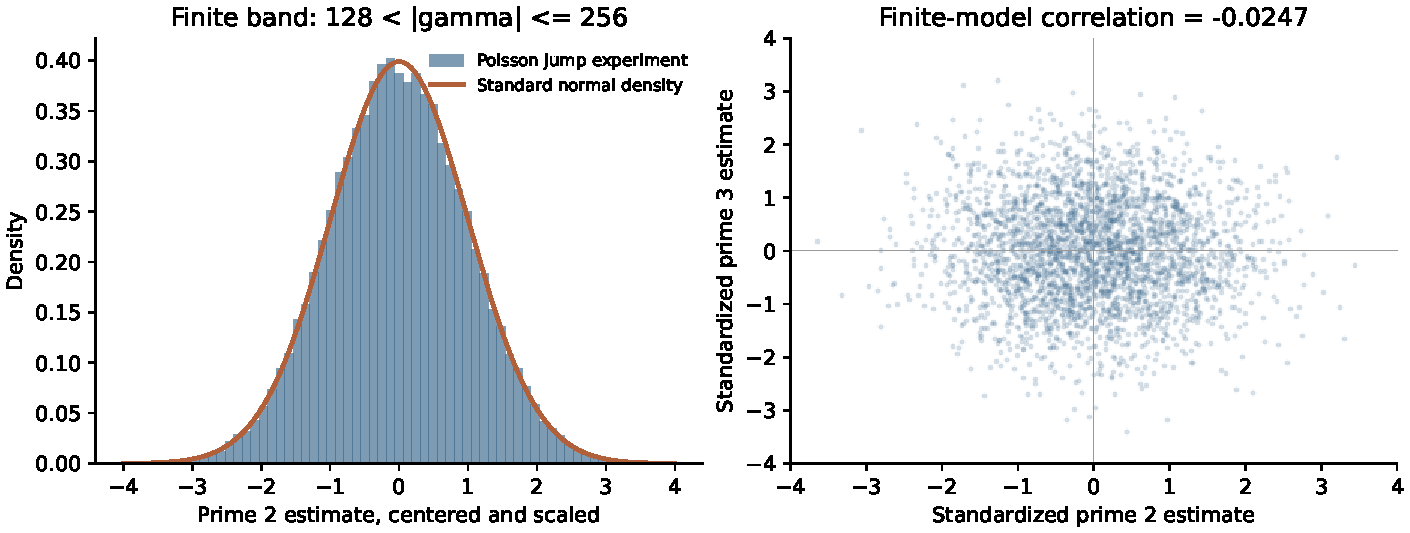
\includegraphics[width=\textwidth]{decoder_illustration.pdf}
\caption{Finite-model illustration from numerical zeta ordinates. Left:
standardized values of the prime-$2$ decoder, with a standard normal density
for comparison. Right: the prime-$2$ and prime-$3$ statistics. This finite
experiment illustrates the Gaussian limit; it neither proves the limit nor
certifies a theorem about the numerical zero fixture.}
\label{fig:illustration}
\end{figure}

\section{Scope, novelty, and proof status}
\label{sec:scope}

\paragraph{What the arithmetic input does.}
The unconditional fixed-$x$ Landau formula reads the sum of $x^\rho$.
Dirichlet GRH turns that summand into the bounded phase
$\sqrt x\,e^{i\gamma\log x}$ that can be evaluated from the jump amplitude.
Without this substitution, the ordinate-defined process does not directly
expose the real parts of the zeros. GRH is used precisely in
Lemma~\ref{lem:landau} and its consequences. The process construction,
entire densities, heat comparison, and finite-grid equivalence use only
ordinary zero counting.

\paragraph{Relation to earlier work.}
Nakamura and Suzuki~\cite{NakamuraSuzuki} relate RH to infinitely divisible
distributions built from zero data. Their measure uses a different
ordinate-based construction; the idea of using infinitely divisible laws in
the study of RH is not new. The equal-mass Cayley-angle process and the
all-order heat expansion are already in the supplied ProveIt article.
Banks~\cite{Banks} supplies the analytic prime-frequency input and studies
differences between zero multisets. The new observation here is that a random
Poisson recording over fixed time retains enough of those prime-frequency
signals for almost-sure arithmetic identification, with the exact Gaussian
noise scale and an explicit information bound.

The inspected article does not contain the decoder~\eqref{eq:decoder}, the
path-law dichotomy, or the finite-grid/path comparison proved here. Searches
for the combination of Li coefficients, Cayley-angle \Levy\ processes,
Dirichlet-character identification and path singularity found no matching
statement. This supports treating the displayed results as a proposed new
contribution relative to the inspected material; it does not certify global
bibliographic priority.

\paragraph{Limitations and what is not asserted.}
The statistical formulas hold for each fixed conductor, character, duration,
and finite set of probe primes; the constants in the error terms are not
claimed to be uniform as these parameters grow. The information lower bound
is not an optimality theorem. Exact recovery from a path uses infinitely many
small jumps with exact amplitudes. The finite-band confidence and testing
bounds describe a concrete finite observation experiment, but an efficient
reconstruction algorithm from noisy, discretely sampled positions would need
additional work. The symmetrization loses precisely the distinction between
$\chi$ and $\bar\chi$; that loss is intrinsic to this process.

\paragraph{Verification status.}
This is a human-readable proof using the explicitly stated Dirichlet-GRH
input, Landau's formula, zero counting, character orthogonality, and elementary
Poisson identities. The new results have not been machine-checked in Lean.
No finite experiment is used to prove an asymptotic assertion. In particular
the factors of two in the construction were retained explicitly: the band
mass is asymptotic to $T\log T/\pi$, the cosine-square mass to
$T\log T/(2\pi)$, and the Hellinger affinity is $e^{-tH_T/2}$.

\begin{thebibliography}{9}
\raggedright
\interlinepenalty=10000

\bibitem{ProveItArticle}
ProveIt Contributors,
\emph{Beyond the Riemann hypothesis for Dirichlet $L$-functions:
consequences, transfers and limits},
26 November 2026, inspected at commit
\texttt{3d8689ceae} (full commit pinned in the link).
In particular \texttt{Article/sections/li.tex},
\texttt{li:sec:univ}, and \texttt{Article/sections/rec.tex}.
\href{https://github.com/VladimirReshetnikov/ProveIt/tree/3d8689ceae76501a5c50f67da37e85369aac4fb6/Analysis/GeneralizedRiemannHypothesis/Article}{Pinned article source}.

\bibitem{LeanSource}
\texttt{lsernau/grh-lean}, readable Lean development,
commit \texttt{72fead102f} (full commit pinned in the link),
vendored in ProveIt under
\path{Analysis/GeneralizedRiemannHypothesis/vendor/grh-lean/grh}.
\href{https://github.com/lsernau/grh-lean/tree/72fead102f663d5c7a407964a13dc0cf9d977207/grh}{Pinned readable Lean source}.

\bibitem{Banks}
W.~D. Banks,
\emph{Comparing zeros of distinct Dirichlet $L$-functions},
Publicationes Mathematicae Debrecen \textbf{106} (2025), 327--335.
\href{https://doi.org/10.5486/PMD.2025.9899}{doi:10.5486/PMD.2025.9899}.
Preprint: \url{https://arxiv.org/abs/2302.07073};
Theorem 1.2 of version 2 gives the Landau formula used here.

\bibitem{BennettEtAl}
M.~A. Bennett, G. Martin, K. O'Bryant and A. Rechnitzer,
\emph{Counting zeros of Dirichlet $L$-functions},
Mathematics of Computation \textbf{90} (2021), 1455--1482.
\href{https://doi.org/10.1090/mcom/3599}{doi:10.1090/mcom/3599}.

\bibitem{Sutherland}
A.~V. Sutherland,
\emph{Verification files for the shorter Lean proof of RH and of GRH for
Dirichlet $L$-functions}, updated 27 November 2026, 17:27 UTC.
\url{https://math.mit.edu/~drew/shortgrh/}.
Accessed 27 November 2026; the page identifies upstream commit
\texttt{72fead10} and reports all checks finished.

\bibitem{NakamuraSuzuki}
T.~Nakamura and M.~Suzuki,
\emph{On infinitely divisible distributions related to the Riemann hypothesis},
Statistics \& Probability Letters \textbf{201} (2023), 109889.
\href{https://doi.org/10.1016/j.spl.2023.109889}{doi:10.1016/j.spl.2023.109889}.
\url{https://arxiv.org/abs/2306.08317}.

\end{thebibliography}
\end{document}
